\documentclass[journal]{IEEEtran}
\usepackage{amsmath,amsfonts,amssymb,amsthm,bm}
\usepackage{booktabs,tabularx}
\usepackage{tikz}
\usetikzlibrary{shapes.geometric,arrows.meta,positioning}
\usepackage{hyperref}

\newtheorem{theorem}{Theorem}
\newtheorem{definition}{Definition}
\newtheorem{remark}{Remark}

\title{Scale-Invariant Contraction Hierarchies: Group-Theoretic Cohesion, Coupling Augmentation, and Compactness Propagation}
\author{Richard~Sherman,~\IEEEmembership{Member,~IEEE}%
\thanks{R. Sherman is with the System Architecture Invariant Manifest Group, Keller, TX 76248 USA.}}

\begin{document}
\maketitle

\begin{abstract}
Multi-area inverter-dominated power grids and autonomous multi-agent swarms exhibit structural self-similarity across fast device, intermediate cluster, and slow supervisory timescales. This paper formalizes a scale-invariant control theory built on four pillars: (1) finite symmetry group equivariance characterizing allowable cohesive configurations ($\mathbf{C}_\ell$) versus symmetry-breaking external coupling interfaces ($\mathbf{P}_\ell$), together with state augmentation converting coupling into internal cohesion; (2) a Renormalization Group (RG) formulation of top-level reserve margin ($\Delta P_{\text{crit}} > 0$) balancing economic cost minimization ($J_{\text{cost}}$) against disruption minimization ($J_{\text{disrupt}}$); (3) time-reversible adjoint flows and stroboscopic singular perturbation lifting continuous dynamics to Nekrashevych self-similar discrete-event trees; and (4) inductive preservation of closedness and compactness across all contracting layers, contrasted with fractal reachable boundaries in the unstable odometer regime.
\end{abstract}

\section{Explicit Trajectory Dynamics: Cohesion vs. Coupling}
Consider an $L$-layer hierarchical network evolving over continuous time $t \in \mathbb{R}_{\ge 0}$. At layer $\ell \in \{1, \dots, L\}$, the network comprises $N_\ell$ interconnected nonlinear subsystems. For every subsystem $i \in \{1, \dots, N_\ell\}$, the local state $x_{\ell,i}(t) \in \mathbb{R}^{n_\ell}$ obeys:
\begin{equation}
\dot{x}_{\ell,i}(t) = f_{\ell,i}\big(x_{\ell,i}(t), x_{\ell,\mathcal{N}_i}(t), \hat{\theta}_{\ell,i}(t)\big) + B_{\ell,i} u_{\ell,i}(t) + E_{\ell,i} v_{\ell,i}(t) + \Delta_{\ell,i} w_{\ell,i}(t)
\end{equation}
where $u_{\ell,i}(t)$ is the local control input, $v_{\ell,i}(t)$ is an exogenous interface input from external modules, and $w_{\ell,i}(t)$ is an $L_2$-bounded disturbance. Stacking all $N_\ell$ subsystems yields the full layer-$\ell$ state vector $x_\ell(t) = (x_{\ell,1}(t), \dots, x_{\ell,N_\ell}(t)) \in \mathcal{X}_\ell \subset \mathbb{R}^{N_\ell n_\ell}$, where a trajectory at layer $\ell$ is an absolutely continuous map $x_\ell : [0, \infty) \to \mathcal{X}_\ell$.

\begin{definition}[Cohesion Symmetry Group and Allowable Configurations]
Let $\mathcal{G}_\ell \le S_{N_\ell}$ be the subgroup of subsystem permutations $P_g$ that preserve the layer-$\ell$ internal interaction matrix $\mathbf{C}_\ell$, i.e., $P_g \mathbf{C}_\ell P_g^\top = \mathbf{C}_\ell$ for all $g \in \mathcal{G}_\ell$. When $v_\ell \equiv 0$, the layer-$\ell$ dynamics are $\mathcal{G}_\ell$-cohesive if permuting states, inputs, and parameters commutes with the vector field:
\begin{equation}
f_\ell(P_g x_\ell, P_g u_\ell, P_g \hat{\theta}_\ell) = P_g f_\ell(x_\ell, u_\ell, \hat{\theta}_\ell), \qquad \forall g \in \mathcal{G}_\ell.
\end{equation}
Thus, $\mathbf{C}_\ell$ and $\mathcal{G}_\ell$ define the set of \emph{allowable configurations} preserving internal network coherence.
\end{definition}

\begin{definition}[External Interface Coupling]
An interaction is termed \emph{coupling} ($\mathbf{P}_\ell$) when subsystem $i$ receives an exogenous signal $v_{\ell,i}(t) = h_{\ell,i}(y_{\text{ext}}(t))$ generated by an external module or synchronization channel (such as a Phase-Locked Loop or range-sensor lag) whose dynamics lie outside $\mathcal{X}_\ell$, thereby breaking $\mathcal{G}_\ell$-equivariance:
\begin{equation}
P_g E_\ell v_\ell(t) \neq E_\ell v_\ell(t) \quad \text{for at least one } g \in \mathcal{G}_\ell.
\end{equation}
\end{definition}

\begin{figure*}[!t]
\centering
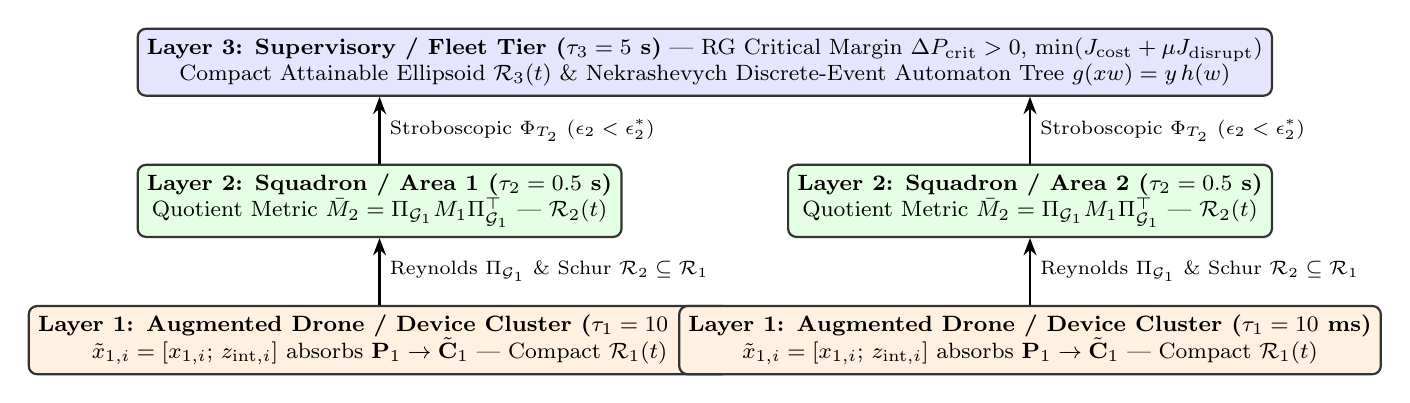
\begin{tikzpicture}[
    node distance=0.6cm and 1.1cm,
    box/.style={rectangle, draw=black!80, thick, rounded corners=3pt, align=center, minimum height=0.85cm, font=\footnotesize},
    l3/.style={box, fill=blue!10, minimum width=12.4cm},
    l2/.style={box, fill=green!10, minimum width=5.6cm},
    l1/.style={box, fill=orange!12, minimum width=5.6cm},
    arr/.style={-{Stealth[length=2.2mm]}, thick}
]
\node[l3] (fleet) {\textbf{Layer 3: Supervisory / Fleet Tier ($\tau_3 = 5\text{ s}$)} --- RG Critical Margin $\Delta P_{\text{crit}} > 0$, $\min (J_{\text{cost}} + \mu J_{\text{disrupt}})$\\Compact Attainable Ellipsoid $\mathcal{R}_3(t)$ \& Nekrashevych Discrete-Event Automaton Tree $g(xw) = y\,h(w)$};

\node[l2, below=0.85cm of fleet.south west, anchor=north west] (sq1) {\textbf{Layer 2: Squadron / Area 1 ($\tau_2 = 0.5\text{ s}$)}\\Quotient Metric $\bar{M}_2 = \Pi_{\mathcal{G}_1} M_1 \Pi_{\mathcal{G}_1}^\top$ | $\mathcal{R}_2(t)$};
\node[l2, below=0.85cm of fleet.south east, anchor=north east] (sq2) {\textbf{Layer 2: Squadron / Area 2 ($\tau_2 = 0.5\text{ s}$)}\\Quotient Metric $\bar{M}_2 = \Pi_{\mathcal{G}_1} M_1 \Pi_{\mathcal{G}_1}^\top$ | $\mathcal{R}_2(t)$};

\node[l1, below=0.85cm of sq1] (dr1) {\textbf{Layer 1: Augmented Drone / Device Cluster ($\tau_1 = 10\text{ ms}$)}\\$\tilde{x}_{1,i} = [x_{1,i};\, z_{\text{int},i}]$ absorbs $\mathbf{P}_1 \to \tilde{\mathbf{C}}_1$ | Compact $\mathcal{R}_1(t)$};
\node[l1, below=0.85cm of sq2] (dr2) {\textbf{Layer 1: Augmented Drone / Device Cluster ($\tau_1 = 10\text{ ms}$)}\\$\tilde{x}_{1,i} = [x_{1,i};\, z_{\text{int},i}]$ absorbs $\mathbf{P}_1 \to \tilde{\mathbf{C}}_1$ | Compact $\mathcal{R}_1(t)$};

\draw[arr] (dr1.north) -- node[right, font=\scriptsize] {Reynolds $\Pi_{\mathcal{G}_1}$ \& Schur $\mathcal{R}_2 \subseteq \mathcal{R}_1$} (sq1.south);
\draw[arr] (dr2.north) -- node[right, font=\scriptsize] {Reynolds $\Pi_{\mathcal{G}_1}$ \& Schur $\mathcal{R}_2 \subseteq \mathcal{R}_1$} (sq2.south);
\draw[arr] (sq1.north) -- node[right, font=\scriptsize] {Stroboscopic $\Phi_{T_2}$ ($\epsilon_2 < \epsilon_2^*$)} (fleet.south -| sq1.north);
\draw[arr] (sq2.north) -- node[right, font=\scriptsize] {Stroboscopic $\Phi_{T_2}$ ($\epsilon_2 < \epsilon_2^*$)} (fleet.south -| sq2.north);
\end{tikzpicture}
\caption{Scale-invariant three-tier contraction hierarchy illustrated on a 3-tier Autonomous Drone Swarm (\texttt{Drone -> Squadron -> Fleet}) and isomorphic multi-area grid. State augmentation converts external coupling $\mathbf{P}_1$ into internal cohesion $\tilde{\mathbf{C}}_1$, while Reynolds projection, stroboscopic lifting, and Schur-complement inclusion propagate compactness upward.}
\label{fig:scale_invariant_arch}
\end{figure*}

We distinguish the static algebraic \emph{cohesive configuration subspace} $\mathcal{X}_\ell^{\mathcal{G}_\ell} \triangleq \{x_\ell \in \mathcal{X}_\ell \mid P_g x_\ell = x_\ell \;\forall g \in \mathcal{G}_\ell\}$ from dynamic \emph{temporal synchronization}, which holds when $\lim_{t \to \infty} d_{M_\ell}(x_\ell(t), \mathcal{X}_\ell^{\mathcal{G}_\ell}) = 0$. Let $\Pi_{\mathcal{G}_\ell} x_\ell = \frac{1}{|\mathcal{G}_\ell|} \sum_{g \in \mathcal{G}_\ell} P_g x_\ell$ denote the Reynolds projector onto $\mathcal{X}_\ell^{\mathcal{G}_\ell}$.

\begin{theorem}[Quotient Contraction Isomorphism]
If layer $\ell$ admits a $\mathcal{G}_\ell$-invariant separable Riemannian metric $M_\ell(x_\ell, \hat{\theta}_\ell)$ ($P_g M_\ell P_g^\top = M_\ell$) with exponential contraction rate $\lambda_\ell > 0$, then: (1) $\mathcal{X}_\ell^{\mathcal{G}_\ell}$ is forward invariant and all trajectories $x_\ell(t)$ synchronize exponentially to $\mathcal{X}_\ell^{\mathcal{G}_\ell}$ as $t \to \infty$; and (2) the renormalized quotient metric $\bar{M}_{\ell+1} = \Pi_{\mathcal{G}_\ell} M_\ell \Pi_{\mathcal{G}_\ell}^\top$ preserves the exact separable Linear Matrix Inequality (LMI) structure at layer $\ell+1$.
\end{theorem}

\section{Renormalization Group Objectives and Coupling Augmentation}
In statistical physics, a Renormalization Group (RG) transformation $V'(\Phi) = \mathcal{R}V(\Phi)$ coarse-grains short-range lattice interactions into macroscopic potentials near a critical temperature $(T - T_c)^\alpha$. In our hierarchy (Fig.~\ref{fig:scale_invariant_arch}), the top layer ($\ell = L$) regulates a critical reserve margin $\Delta P_{\text{crit}} \triangleq P_{\text{deliver}} - P_{\text{demand}} > 0$ while jointly minimizing two supervisory objectives:
\begin{equation}
\min_{u} \; \Big( J_{\text{cost}}(u) + \mu\, J_{\text{disrupt}}(x, u) \Big)
\end{equation}
where $J_{\text{cost}}$ captures fuel, generation, and curtailment costs, and $J_{\text{disrupt}}$ penalizes physical disruptions such as collisions, relay trips, and mode-shift chattering.

\begin{remark}[Converting External Coupling Into Internal Cohesion]
Whenever an exogenous coupling channel $v_{\ell,i} = h_{\ell,i}(y_{\text{ext}})$ is governed by finite-dimensional interface dynamics $\dot{z}_{\text{int},i} = q_{\ell,i}(z_{\text{int},i}, x_{\ell,i}, x_{\ell,\mathcal{N}_i})$, augmenting the local state to $\tilde{x}_{\ell,i} = [x_{\ell,i};\, z_{\text{int},i}]$ absorbs the external input into an internal state transition, transforming the coupled network $(\mathbf{C}_\ell, \mathbf{P}_\ell)$ into a purely cohesive augmented system $\tilde{\mathbf{C}}_\ell$.
\end{remark}

\section{Time-Reversible Adjoints and Continuous-to-Discrete Lifting}
Because smooth vector fields $f_\ell$ generate local diffeomorphic flows $\phi_t^\ell$ whose variational adjoint equations $\dot{\psi}_\ell(t) = -A_\ell(x_\ell(t))^\top \psi_\ell(t)$ integrate backward in time, continuous trajectory transformations are invertible, justifying modeling hierarchical symmetry actions by an invertible \emph{group} $G$. Following Nekrashevych~\cite{nekrashevych05}, let $X$ be a finite alphabet indexing subsystems and $X^*$ be the rooted tree of hierarchical address words $w = x_1 \cdots x_k$. Along the unique contracting nominal trajectory $x^*(t)$, a self-similar action of $G$ satisfies $g(xw) = y\,h(w)$ for all $g \in G$, $x \in X$, and $w \in X^*$.

To bridge continuous dynamics at layer $\ell$ to discrete-event transitions at layer $\ell+1$, singular perturbation ($\epsilon_\ell = \tau_\ell / \tau_{\ell+1} \ll 1$) separates fast and slow \emph{continuous} states within a cohesive tier, while the stroboscopic sampled-data (Poincar\'e) return map:
\begin{equation}
x_{\ell+1}[k+1] = \Phi_{T_\ell}\big(x_{\ell+1}[k],\, x_\ell(t_k + T_\ell)\big)
\end{equation}
lifts the settled fast continuous boundary layer over macro-interval $T_\ell$ into a discrete-event transition tree governed by the Mealy automaton $(G, X)$.

\section{Preservation of Closedness, Compactness, and Chaotic Fractals}
For general nonlinear systems, forward attainable sets are neither closed nor compact. However, when layer $\ell = 1$ enforces metric coercivity $M_1(\hat{\theta}_1) \succeq \alpha_1 I \succ 0$ and finite $L_2$ gain $\gamma_1 < \infty$, its Pontryagin attainable set $\mathcal{R}_1(t)$ is closed and bounded (hence compact by Heine--Borel).

\begin{theorem}[Inductive Preservation of Closedness and Compactness]
If $\mathcal{R}_1(t)$ is closed and compact at Layer~1, every upward projection $\Pi_{\ell \to \ell+1}$ is continuous, and adjacent layers satisfy the Schur-complement containment LMI:
\begin{equation}
\frac{1}{\rho_{\ell+1}^2} M_{\ell+1}(\hat{\theta}_{\ell+1}) \succeq \frac{1}{\rho_\ell^2} \Pi_{\ell+1 \to \ell}^\top M_\ell(\hat{\theta}_\ell) \Pi_{\ell+1 \to \ell},
\end{equation}
then $\mathcal{R}_\ell(t)$ remains closed and compact at every higher layer $\ell = 2, \dots, L$.
\end{theorem}

\begin{remark}[Chaotic Odometer Regime and Fractal Attainable Sets]
When contraction fails ($\lambda_{\text{eff}} \le 0$) and unabsorbed disturbances trigger the infinite-order adding-machine (runaway clock) automaton $a(1w) = 0\,a(w)$, trajectories repeatedly fold against physical saturation rails, fragmenting the reachable boundary into a Cantor-like fractal limit set of non-integer Hausdorff dimension~\cite{nekrashevych05}.
\end{remark}

\begin{thebibliography}{9}
\bibitem{nekrashevych05} V. Nekrashevych, \textit{Self-Similar Groups}, Mathematical Surveys and Monographs, vol. 117. Providence, RI, USA: Amer. Math. Soc., 2005.
\end{thebibliography}

\end{document}
